\documentclass{svproc}
%\documentclass{article}
\def\UrlFont{\rmfamily}
\usepackage{graphicx}
%\usepackage{subcaption}
\usepackage{bm}
%\usepackage{geometry}
\usepackage{float}
\usepackage{caption}
\usepackage{pdfpages}
\usepackage{setspace}
\usepackage{amsmath}
\usepackage{amssymb}
\usepackage{multicol}
\usepackage{color}
\doublespacing
\usepackage[margin=1.1in]{geometry}% to typeset URLs, URIs, and DOIs
\usepackage{url}
\usepackage{threeparttable}
\usepackage[bottom]{footmisc}
\usepackage{adjustbox}
\usepackage{multirow}
\usepackage{makecell}
\usepackage{caption}
\usepackage{subfig}
\def\UrlFont{\rmfamily}
\raggedbottom
\newenvironment{centermath}
 {\begin{center}$\displaystyle}
 {$\end{center}}
\newcommand\scalemath[2]{\scalebox{#1}{\mbox{\ensuremath{\displaystyle #2}}}}



\begin{document}
\mainmatter              % start of a contribution
%


\title{Solar Analysis}
%
\titlerunning{Solar Analysis}  % abbreviated title(for running head)
%                                     also used for the TOC unless
%                                     \toctitle is used
%
\author{Jacob Merrell}

\institute{}
%
%%%% list of authors for the TOC(use if author list has to be modified)

\maketitle  

\begin{abstract}
   Solar energy is environmentally friendly, but can it also be cost efficient? This study focuses on power bill data collected from one solar panel owner. The study confirms that solar power helps save money, and hypothesizes that on average the savings from using the solar panel after 8 years will cover the costs of the installation. We explore ways to account for the correlation in the data, and to also incorporate temperature into the model.   
\end{abstract}

\section{Introduction}

Ideally energy would be efficient, cheap, and environmentally friendly. Finding the right balance is a difficult question for scientists to answer. Sunlight is available to all, given the weather is right. Harnessing the power of solar energy is an environmentally friendly alternative to other more pollutant producing energy sources. The purpose of this analysis to be able to: (1) predict how much power bills are going to be in the future (2) how much can someone save, on average, using solar energy, and (3) how long it will take to earn back the money used to install solar equipment. Regression techniques to handle correlated data will be used to answer the goals of the analysis.

\section{Exploratory Data Analysis}

\begin{center}
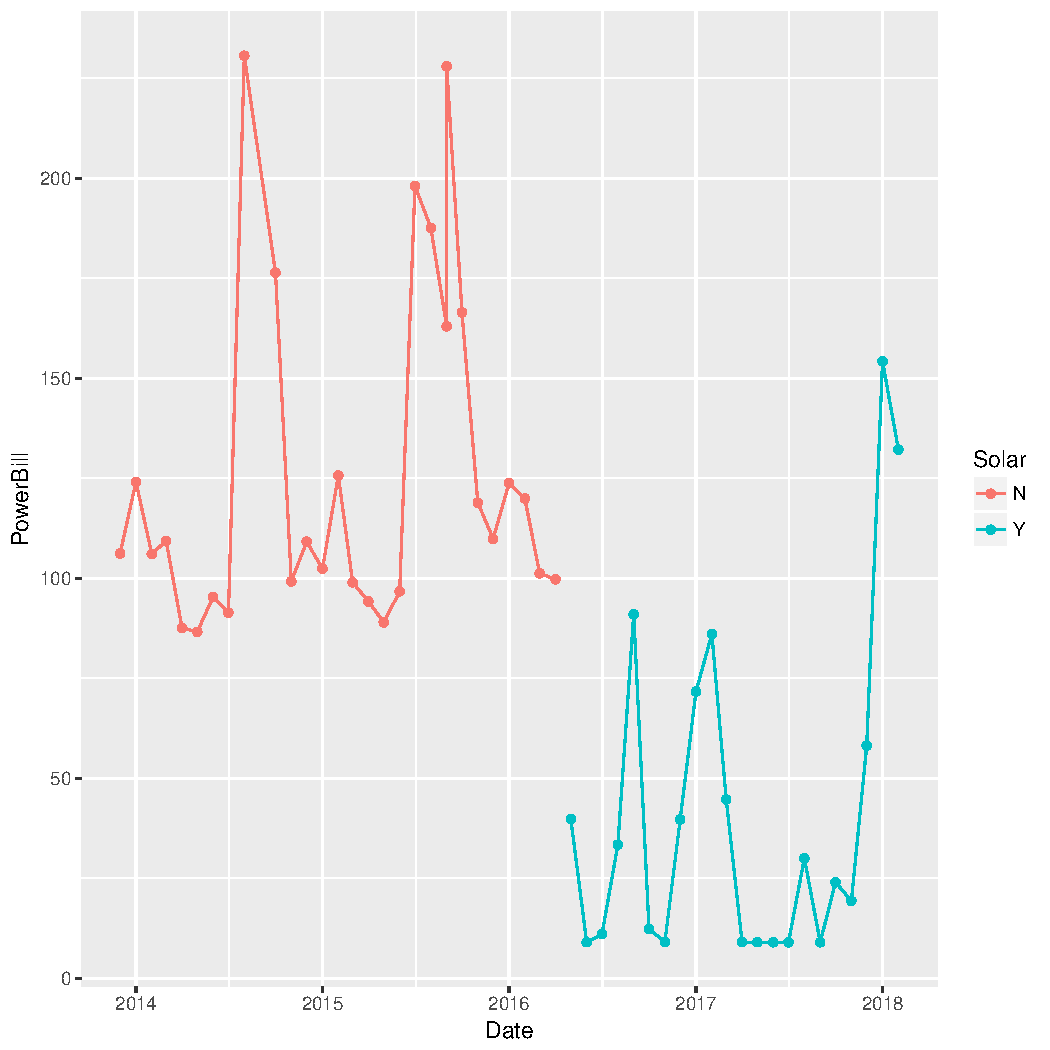
\includegraphics [height=7.5cm]{solar_data.pdf}
\end{center}

The graph above shows the power bill for the subject given dates in time. There is a sizable difference between the power bill after switching to solar energy. Exploring the data shows that normal regression methods are inadequate for this data. There appears to be a seasonal trend in the power bill. This makes sense because in very cold and very hot months, more energy is used to maintain the climate inside the home. The dataset includes 51 months of power bills from the same subject. 

\section{Model Selection}

The model used for this analysis is 

\begin{equation}
 Y \sim N(X\beta, \sigma^2R)
\end{equation}

In the model $Y$ denotes the vector of power bill amounts, and the $X$ matrix contains the observed values of the explanatory variables at the date of each power bill. The $\beta$ vector contains the model coefficients, $\sigma^2$ is the variance of the residuals, and $R$ is the variance covariance matrix. The variance covariance matrix in this model is structured as AR(1). This model assumes that correlation of each observation with the previous observation is constant and equal to $\rho$. This makes sense to use an AR(1) model since the data are measured in discrete and consistent time intervals.

The effects being measured in the model are solar v non-solar power bills, the interaction between solar status and season (summer or winter), and the interaction between season and temperature. Temperature was not originally given in the dataset, but was gathered from the US Climate Data website. The reason for gathering this data was to see the effect extreme temperatures had on the power bill.

The model assumptions are normality of the standardized residuals, homoscedacisity, and that the data are multivariate normally distributed. Normality of the residuals can be observed by plotting the residuals to verify if they seem normally distributed. Homoscedacisity is verified through a graph of the fitted values v. the residuals. A constant variability or jitter of the residual values about 0 should be similar across all fitted values. The model follows multivariate normal distribution. 

The model will help us achieve our goals by estimating coefficients and allowing us to make predictions of the power bill amount at each month. The model will also help us capture the seasonality trends inherent in the data.




\section{Model Justification}
Since the data are correlated, using the residuals from the model without any adjustment can lead to incorrect conclusions about the assumptions. To correct for this issue, we used a decorrelated regression model. After undergoing the decorrelation transformation, the residuals and fitted values can be used to verify whether or not the assumptions hold. The assumptions for the model are explored in the graphs below

\begin{center}
\includegraphics [height=7.5cm]{assump.pdf}
\end{center}

The histogram of the standardized residuals shows a normal distribution. The fitted v. residual plot shows that the variance of the residuals about the 0 line is about the same. All assumptions hold for this study.

\section{Performance Evaluation}

The model had an adjusted R-squared of 0.9376. This mean 93.76\% of variation in power bill is explained by the model. To test the predictive power of the model, we used test and training data to cross validate. The test and training datasets were chosen to preserve the time series; in this case choosing random points would interfere with the correlated structure inherent in the data. The training data was used to predict the test data. The RMSE, bias, and 95\% prediction interval coverage we calculated. This process was repeated several times to get more reliable results. On average, the RMSE was \$27.21; this means the predictions were off by \$27.21 on average. The 95\% confidence interval for the RMSE was (\$6.74, \$54.48). The bias showed that we were underestimating the power bill by \$0.67 on average, and almost 95\% of all observed power bill values were contained within the prediction intervals. Even though the coverage was very good, the average prediction window was \$104.57. This means most of the predictions for a power bill during a given month would have been in a ballpark of plus or minus \$50 away from the point estimate. 

\section{Results}

The graph below shows the fitted values from the model compared to the actual power bill values.

\begin{center}
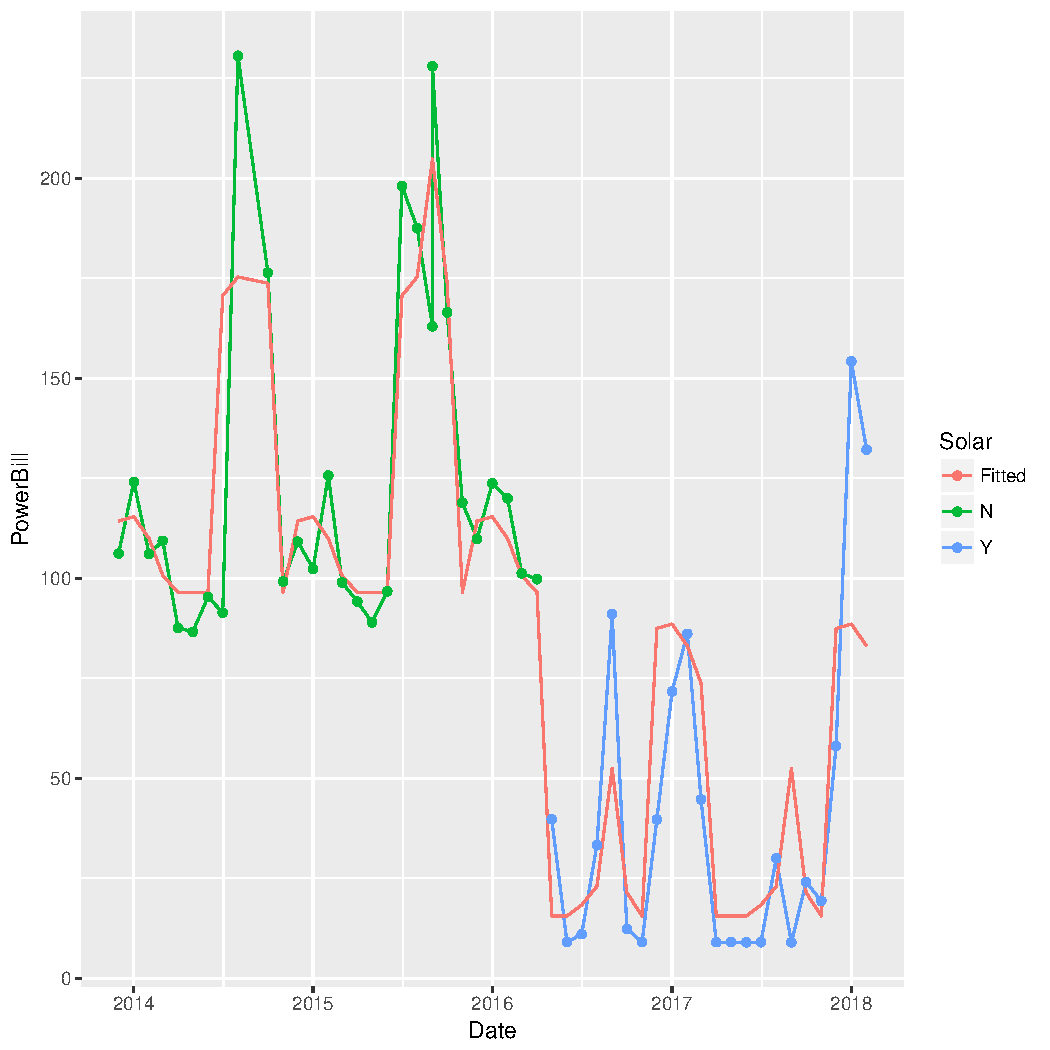
\includegraphics [height=7.5cm]{solar_fit.pdf}
\end{center}

While the model uses an AR(1) covariance structure, the model estimate for $\rho$ is very small (.0377). This means the effects and interactions included in the model account for most of the correlation inherent in the data. To achieve the goals of the study we used the model to predict the amount of money spent on power bills over the next 10 years. Then we compared the amount of money spent per month when using solar power v. the amount of money spent on power when not using solar energy. The average monthly savings when using solar energy is \$86.69. The 95\% confidence interval for the monthly savings is (\$80.41,\$92.97). In this the study, the subject using solar power in their home paid \$8,000 (after government subsidies) to install the solar panels. Assuming the average monthly savings, it would take 7.69 years of cumulative saving to cover the installation costs. The 95\% confidence interval for the amount of time it would take to recover the initial investment is (7.17,8.29).


\section{Conclusion}
Using solar power helps save \$86.69 on average each month. However, the RMSE is fairly given the size of the monthly power bill. Predictions for individual months will vary much more than average yearly totals or average seasonal totals. Assuming an initial \$8,000 investment, it will take 7.69 years on average for the investment in solar panels to pay off. All power bill data in this study was gathered about 1 home owner. One improvement to be made for future studies is to include more solar panel owners across a broad range of geographical locations. Another element not incorporated into the study was the impact of inflation or changing utility costs on the power bill amount. The data overall could have used more explanatory variables to explain the variation in power bill. If one plans on living in their home for an extended period of time, solar energy is a cost effective and nature friendly way of using electricity.

\newpage
\begin{thebibliography}{6}

\bibitem{R}
R: A Language and Environment for Statistical Computing.R Core Team.
R Foundation for Statistical Computing.Vienna, Austria.
(2017).url = {https://www.R-project.org/}


\end{thebibliography}




\end{document}



